\section{Motivação e Contextualização}
A Internet das Coisas, em inglês, \sigla{IoT}{\textit{Internet of Things}}, é um paradigma em ascensão na computação. Ainda sem uma definição estabelecida, IoT se baseia na ideia da interação dos mundos físico e cibernético, através da conexão de dispositivos do nosso dia-a-dia à Internet, de forma que eles possam se comunicar e colaborar para realizar tarefas \cite{Al-Fuqaha2015Internet}. Na sua maioria, os dispositivos IoT serão sensores, microcontroladores e sistemas embarcados --- em suma, sistemas computacionais simples, que gastam pouca energia e possuem limitações de recursos computacionais e de largura de banda \cite{Atzori2010Internet}.

Sendo assim, muito do desenvolvimento desses sistemas se deu pautado justamente na solução dessas limitações técnicas --- de energia, poder computacional, resistência a situações críticas etc. --- deixando de lado, no entanto, um importante aspecto do qualquer sistema computacional: segurança (TODO: REFERÊNCIA). 








\section{Protocolos em IoT e Modelo Publish/Subscribe}

A Internet das Coisas, como o próprio nome dá a entender, faz parte da Internet, ou seja, utiliza as mesmas vias de comunicação que as demais máquinas na rede. No entanto, se alguns protocolos, como o \sigla{TCP}{\textit{Transfer Control Protocol}} e o \sigla{IP}{\textit{Internet Protocol}}, em especial o IPv6, são frequentemente usados por dispositivos IoT, outros, como o \sigla{HTTP}{\textit{HyperText Transfer Protocol}} e sua versão criptografada --- o HTTPS ---, largamente utilizados na camada Web da rede, não o são. Com vistas a manter uma conexão mais leve, consumindo menos energia e recursos computacionais, IoT conta com uma série de protocolos alternativos ao HTTP para troca de mensagens, como por exemplo o MQTT (TODO: REFERÊNCIA).

O modelo \emph{Publish/Subscribe} é um dos modelos de comunicação comumente utilizados por dispositivos IoT, sobretudo em redes de sensores (TODO: REFERÊNCIA). Conforme a \autoref{publish-subscribe}, nesse modelo os clientes --- máquinas que se comunicam --- se conectam a um corretor, ou \emph{broker} em inglês, e se inscrevem (\emph{subscribe}) em tópicos. Os clientes podem ainda publicar (\emph{publish}) mensagens em um ou mais tópicos. Assim, todos os clientes que estiverem inscritos nesses tópicos receberão as mensagens ali publicadas.


\begin{figure}[htb]
 \caption{Modelo Publish/Subscribe}
 \label{publish-subscribe}
 \centering
 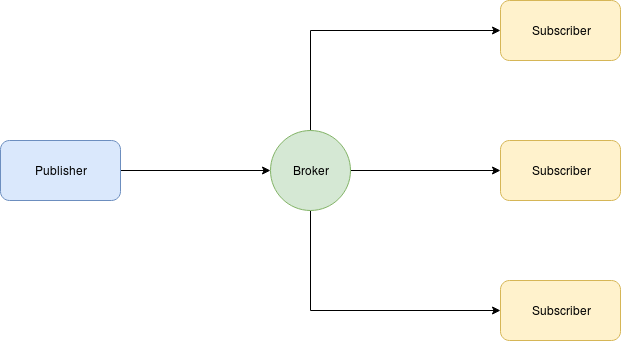
\includegraphics[scale=0.6]{images/publish-subscribe.png}
 \fautor
\end{figure}


Esse modelo permite que o broker despenda uma quantidade maior de recursos energéticos e computacionais --- para armazenar as listas dos clientes inscritos, garantir níveis de qualidade de serviço, enviar publicações para clientes inscritos etc. --- enquanto os clientes somente enviam e recebem as mensagens quando necessário (TODO: REFERÊNCIA -> BUSY WAIT).









\section{Objetivos}

Por conta do desenvolvimento desenfreado das tecnologias IoT, não tendo como objetivo a grande maioria dos aspectos de segurança, logo percebeu-se uma ampla gama de falhas em diversos protocolos de comunicação (TODO: REFERÊNCIA) projetados para esses sistemas, bem como ausência de implementação de criptografia e outras práticas de segurança, tão comuns em outras áreas da computação. Sendo assim, esse trabalho implementa dois ataques que causam negação de serviço em um dos protocolos mais largamente utilizados em dispositivos IoT --- mostrando que, de fato, essas falhas existem e podem ser facilmente exploradas.









\section{Organização}

Esta monografia começa por introduzir brevemente o conceito de Internet das Coisas, com foco no seu desenvolvimento e em como ele afetou os aspectos de segurança da informação nesse meio. Em seguida, apresentamos conceitos e tecnologias importantes que fazem parte do escopo dos ataques a serem implementados. Mostramos a implementação de dois ataques ao protocolo MQTT, comentando brevemente sobre medidas de mitigação e respectivas sofisticações dos ataques para superar essas medidas. Finalmente, apresentamos nossas conclusões sobre o trabalho e comentamos brevemente sobre alguns aspectos do curso de Ciências de Computação no \sigla{ICMC}{Instituto de Ciências Matemáticas e de Computação} do campus de São Carlos da \sigla{USP}{Universidade de São Paulo}.

